\documentclass[a4paper]{article}

\usepackage[utf8]{inputenc}
\usepackage[polish]{babel}
\usepackage{polski}
\usepackage{listings}
\usepackage[T1]{fontenc}
\usepackage[margin=0.9in]{geometry}
\usepackage[usenames,dvipsnames]{xcolor}
\usepackage{lmodern}
\usepackage{pdfpages}
\usepackage{float}
\usepackage{longtable}
\usepackage{graphicx}
\usepackage{pdfpages}
\usepackage{multirow}

\begin{document}

\begin{titlepage}

\newcommand{\HRule}{\rule{\linewidth}{0.5mm}} 

\center 
 
%----------------------------------------------------------------------------------------
%	HEADING SECTIONS
%----------------------------------------------------------------------------------------

\textsc{\LARGE Politechnika Wrocławska}\\[1.0cm] % Name of your university/college
\textsc{\Large Bazy Danych}\\[0.2cm] % Minor heading such as course title
\textsc{\large Raport końcowy}\\[2cm]

%----------------------------------------------------------------------------------------
%	TITLE SECTION
%----------------------------------------------------------------------------------------

\HRule \\[0.4cm]
{ \huge \bfseries Analizator danych pogodowych}\\[0.4cm] % Title of your document
\HRule \\[3cm]
 
%----------------------------------------------------------------------------------------
%	AUTHOR SECTION
%----------------------------------------------------------------------------------------

\begin{minipage}{0.4\textwidth}
\begin{flushleft} \large
\emph{Autorzy:}\\
Aleksandra \textsc{Grzelak}\newline
Dorian \textsc{Janiak}\newline
Marcin \textsc{Ochman}

\end{flushleft}
\end{minipage}
~
\begin{minipage}{0.4\textwidth}
\begin{flushright} \large
\emph{Prowadzący:} \\
dr hab. inż. Grzegorz \textsc{Mzyk}
\end{flushright}
\end{minipage}\\[12cm]

{\large \today}\\[3cm] 


\vfill 

\end{titlepage}

\newpage
\tableofcontents
\listoffigures
\newpage

\section{Opis projektu}
W ramach projektu powstała baza danych zawierająca dane pomiarowe ze stacji pogodowych oraz interfejs graficzny w postaci strony internetowej. Do zrealizowania zadania posłużył serwer \textbf{MySQL} (przetrzymywanie oraz udostępnianie danych), język \textbf{Python} (logika aplikacji) wraz z modułem \textbf{Django} (framework web - strona graficzna oraz zarządzająca bazą). 
\section{Opis funkcjonalności}
Stworzony przez nas analizator realizuje poniżej wymienione funkcje:
\begin{itemize}
	\item \textbf{Wczytywanie danych pogodowych z plików CSV} - plik ma określony format (opisany w punkcie: 8.2). Funkcja uaktywnia się jedynie dla zalogowanych użytkowników aplikacji. Dostępna jest z poziomu panelu sterowania położonego w górnej części strony (''Wczytaj dane''). Wczytuje dane z pliku jednocześnie wpisując je do tabeli \verb Analyzer_danepomiarowe . 
	\item \textbf{Logowanie użytkownika} - logowanie odbywa się z poziomu górnego panelu sterowania (''zaloguj się''). Dane użytkownika domyślnie zapisane są w tabeli \verb auth_user . Jeśli wpisane hasło lub login nie pokryją się z zawartością bazy zostanie wyświetlony monit o niepoprawnym logowaniu. W przeciwnym wypadku logowanie przebiegnie pomyślnie i użytkownik otrzyma dostęp do funkcji wczytywania danych pogodowych. Została zaimplementowana również możliwość wylogowania użytkownika.
	\item \textbf{Rysowanie wykresów} - wykresy rysowane są gdy użytkownik wybierze jedną z opcji związaną z podglądem danych pogodowych. Do rysowania wykorzystywany był przez nas wczesniej pakiet matplotlib. Ze względu na lepszą prezentację danych wybraliśmy jednak pakiet od google \textbf{google.visualization}, z którego można korzystać w wywołaniach \textbf{Java Script}.
	\item \textbf{Wybór stacji i rodzaju danych pomiarowych} - użytkownik wybiera stację oraz parametr, którego wykres chce wyświetlić. W programie po uruchomieniu funkcji reagującej na naciśnięcie odpowiedniego przycisku zostaje stworzony obiekt klasy Algorithm, który zawiera zestaw danych dla wybranej stacji oraz rodzaju pomiaru. 
	\item \textbf{Usuwanie danych pomiarowych} - jeśli użytkownik jest zalogowany ma możliwość z poziomu zakładki ''podgląd stacji pogodowych'' usunąć dane. 
	\item \textbf{Prognoza} - w programie został zaimplementowany algorytm prognozowania. Został on oparty na modelu \textbf{ARMA}. Algorytm nie jest jednak czystym prognozowaniem ARMA, został on zmodyfikowany. W naszej implementacji opiera się on również na interpolacji oraz wyznaczaniu wzmocnień.
\end{itemize}

\section{Struktura aplikacji WEB}
Organizacja aplikacji w dużej mierze została narzucona przez samo Django. Poniżej prezentujemy opis istotnych plików i katalogów:
\begin{itemize}
	\item \textbf{WheatherAnalyzer/settings.py} - plik ten tworzony jest automatycznie przez Django w trakcie inicjalizacji projektu. W tym pliku wpisane są takie informacje jak silnik bazo-danowy, z którego korzystamy, login i hasło użytkownika bazy danych (w momencie przeniesienia bazy na inny komputer należy pamiętać, że jeśli posiada się konto z hasłem do dostępu do bazy danych, należy uzupełnić pola USER oraz PASSWORD. Istotnymi informacjami są również pakiety django, z których korzysta aplikacja.
	\item \textbf{WheatherAnalyzer/urls.py} - plik ten zawiera informacje na temat linków (stron) jakie pojawią się w bazie. Przykładowo:
	\begin{verbatim}
		url(r'^station/(?P<station_id>[0-9]+)/(?P<rodzaj_pom_id>[0-9]+)$',
 	StationsDetailView.as_view(), name="station_detail"),
	\end{verbatim}
Tworzy nowy link, który jest dopasowywany przy użyciu regex i przekierowuje działanie Django do klasy StationsDetailView z pliku view.py. Wartość parametru name posłuży do odwołań z szablonu html. 
	\item \textbf{Analyzer/admin.py} - plik rejestruje modele z pliku models.py. Plik jest wykorzystywany przez panel administracyjny Django. Modele zarejestrowane w tym pliku będą widziane w panelu i będzie można nimi zarządzać.
	\item \textbf{Analyzer/models.py} - plik zawiera modele, które między innymi pozwalają uzyskać dane z tabel baz danych. Modelami są zwykłe klasy, które korzystają z pakietu \textit{django.db}, zarządzającego bazami danych, w celu wyciągania danych z poszczególnych rekordów. Przykładowy kod takiej klasy zaprezentowany został poniżej:
	\begin{verbatim}
	class Stacja(models.Model):
    # id = models.AutoField(primary_key=True)
    nazwa = models.CharField(max_length=30)

    def __unicode__(self):
        return self.nazwa
	\end{verbatim}
pole \textit{name} od tej pory będzie przechowywać nazwę stacji zapisaną przy użyciu typu VARCHAR(30). Stworzenie obiektu takiej klasy owocuje pobraniem rekordu z tabeli Analyzer\_stacje.
	\item \textbf{Analyzer/forms.py} - plik jest wykorzystywany do tworzenia formularzy (np. formularz logowania). Klasy przechowujące formularze muszą odziedziczyć po jednej z klas django.forms lub crispy\_forms. Aby móc użyć formularza z poziomu szablonów należy dla niego najpierw stworzyć link w pliku urls.py i uzupełnić parametr name. 
	\item \textbf{Analyzer/views.py} - plik przechowuje klasy, które służą do rysowania widoku. W każdej z klas należy powiązać klasę z szablonem oraz zaimplementować metody, które zwrócą kontekst w postaci mapy lub same zażądają wyrenderowania widoku funkcją render(). W funkcjach tych korzysta się z modeli zaimplementowanych w pliku models.py, aby pobrać dane i przekazać do django. 
	\item \textbf{templates/analyzer/} - folder zawiera zbiór plików w formacie HTML, które są szablonami stron. Aby sięgnąć po dane z bazy danych lub formularze należy w ich kodzie wywołać odpowiednie funkcje (które były już wcześniej powiązane), przykładowo:
	\begin{verbatim}
	 
       <div id="curve_chart"></div>
    
    	<p> Brak danych do wyświetlenia.</p>
    
	\end{verbatim}
powyższy kod sprawdzi czy istnieją elementy dane\_pom, jeśli tak to wyświetli wykres stworzony w javascript przy użyciu biblioteki google.visualizations. W przeciwnym wypaku wyświetli się napis "Brak danych ...". 
\end{itemize}

\subsection{Modele}
Poniżej znajdują się deklaracje poszczególnych klas oraz krótkie opisy do nich:
\begin{itemize}
	\item \textbf{class Stacja(models.Model)} \newline
	model pobiera dane z bazy \textit{Analyzer\_stacje}.
	Klasa posiada tylko jedno pole \textit{nazwa}, które odpowiada nazwie stacji.
	\item \textbf{class Jednostka(models.Model)} \newline
	model pobiera dane z bazy \textit{Analyzer\_jednostka}.
	Klasa posiada tylko jedno pole \textit{nazwa}, które odpowiada nazwie jednostki.
	\item \textbf{class RodzajPomiaru(models.Model)} \newline
	model pobiera dane z bazy \textit{Analyzer\_rodzajpomiaru}.
	Klasa posiada dwa pola: \textit{nazwa}, które odpowiada nazwie rodzaju pomiaru oraz \textit{jednostka}, które przechowuje klucz obcy z tabeli jednostek. 
	\item \textbf{class DanePomiarowe(models.Model)} \newline
	model pobiera dane z bazy \textit{Analyzer\_danepomiarowe}.
	Klasa posiada pola: \textit{wartosc}, która jest reprezentowana przez typ całkowity, \textit{rodzaj\_pomiaru} oraz \textit{stacja}, które są kluczami obcymi, \textit{data} reprezentowana w formacie datetime.datetime.
\end{itemize}

\subsubsection{Klasa Algorithm}
Klasa posiada więcej niż jedną funkcję i nie realizuje tylko funkcji uzyskiwania dostępu do rekordu tabeli. 
Poniżej opisane zostały funkcje, które zostały zaimplementowane w klasie:
\begin{itemize}
	\item \textbf{\_\_init\_\_(self, dlugosc\_prognozy, stacja\_id, rodzaj\_pomiaru)}
	\begin{itemize}
		\item self - standardowy argument w języku Python pozwalający na korzystanie z pól i funkcji klasy
		\item dlugosc\_prognozy - ile dni ma byc prognozowane w formacie całkowitej liczby
		\item stacja\_id - numer id, który posłuży do pobrania obiektu reprezentującego rekord stacji
		\item rodzaj\_pomiaru - numer id, który posłuży do pobrania obiektu reprezentującego rekord rodzaju pomiaru
	\end{itemize}
	Konstruktor pobiera dane z bazy danych przy użyciu obiektu klasy \textit{DanePomiarowe} oraz funkcji filter. Następnie przygotowuje zestawienie dat i wartości pomiarów w strukturze dta, która jest wykorzystywana przez kolejne funkcje. 

	\item \textbf{wyznaczPiQ(self,dane)}
	\begin{itemize}
		\item dane - same wartości pomiarów
	\end{itemize}
	Funkcja wyznacza parametry P (na podstawie PACF) oraz Q (na podstawie ACF). 

	\item \textbf{minimalizujPiQ(self,p,q)}
	\begin{itemize}
		\item p - parametr P w postaci liczby całkowitej
		\item q - parametr Q w postaci liczby całkowitej
	\end{itemize}
	Funkcja ogranicza parametry P i Q do wartości maksymalnej 20 jeśli przekraczają tę granicę. Stara się zachować proporcje między parametrami. 

	\item \textbf{artistico\_usrednijWykres(self, dane,rzad,ileNowych)}
	\begin{itemize}
		\item dane - pełne dane z datami oraz wartościami
		\item rzad - rząd interpolacji
		\item ileNowych - liczba wskazująca na ile dni ma zostać stworzona predykcja
	\end{itemize}
	Funkcja interpoluje oryginalne dane w zakresie od pierwszej dostępnej daty do ostatniej + ileNowych

	\item \textbf{artistico\_odejmijTrend(self,daneOryg,trend)}
	\begin{itemize}
		\item daneOryg - pełne dane z datami oraz wartościami 
		\item trend - wartości, które mają zostać odjęte
	\end{itemize}
	Funkcja zwraca tablicę różnic danych oryginalnych z danymi uśrednionymi

	\item \textbf{artistico\_obliczWzmocnienie(self,dane,predykcja,trend,ileBracPodUwage)}
	\begin{itemize}
		\item dane - pełne dane z datami oraz wartościami
		\item predykcja - wartości prognozowane otrzymane w wyniku dopasowania modelu ARMA
		\item trend - uśrednione wartości oryginalnych danych
		\item ileBracPodUwage - liczba całkowita informująca ile ostatnich pomiarów ma zostać uwzględnione przy obliczaniu wzmocnień
	\end{itemize}
	Funkcja wyznacza minimalne i maksymalne wartości dla zakresu \textit{ileBracPodUwage} pomiarów predykcji oraz oryginalnych danych. Następnie wylicza między nimi wzmocnienie i przemnażając uzyskane wartości predykcji otrzymuje odpowiednio przeskalowane wartości predykcji. 

	\item \textbf{mainAlg(self)}\newline
	W funkcji znajduje się główna część algorytmu predykcji. Najpierw wyznacza wartości interpolowane oryginalnych danych (z względnie małym rzędem). Następnie odejmuje te wartości od oryginalnych danych. Na podstawie oryginalnych danych, współczynników AIC oraz wyznaczonych maksymalnych parametrów P i Q na podstawie funkcji autokorelacji, wyznacza model ARMA. Następnie, aby pozbyć się dużych wahań temperatury wylicza wzmocnienia na bazie oryginalnych danych i wahań uzyskanych wcześniej. Rezultaty pozostawia w tablicach x\_prediction oraz preds.
\end{itemize}
\subsection{Formularze}
Zawartość formularzy definiowana jest w ich konstruktorach. Nasza aplikacja posiada dwa formularze: 
\begin{itemize}
	\item \textbf{LoginForm(AuthenticationForm)}\newline
	Formularz dziedziczy po szablonie AuthenticationForm z pakietu django.contrib.auth.forms, ale korzysta z elementów formularza FormHelper dostępnego w pakiecie crispy\_forms. W formularzu zdefiniowane zostały pola ''username'', ''password'' oraz przycisk ''Zaloguj'' (korzysta z klasy Submit).
	\item \textbf{LoadFilenameForm(forms.Form)}\newline
	Formularz dziedziczy po szablonie Form dostępnym w pakiecie django.forms. W formularzu zdefiniowane zostało pole ''file'' oraz przycisk ''Wczytaj'' (korzysta z klasy Submit). 
\end{itemize}

\subsection{Widoki}
Obsługa widoków może się opierać zarówno na Klasach jak i funkcjach. Poniżej zostały one opisane:
\begin{itemize}
	\item \textbf{IndexView(TemplateView)}\newline
	Klasa jedynie rejestruje szablon, reprezentujący stronę główną.
	\item \textbf{LoginView(FormView)}\newline
	Klasa rejestruje szablon, reprezentujący stronę logowania (''analyzer/login.html''). 
	\item \textbf{LogoutView(TemplateView)}\newline
	Klasa rejestruje szablon, reprezentujący stronę wylogowania (''analyzer/logout.html''). 
	\item \textbf{StationsView(TemplateView)}\newline
	Klasa rejestruje szablon, reprezentujący stronę listy stacji (''analyzer/stations.html''). 
	\item \textbf{StationsDetailView(TemplateView)}\newline
	Klasa rejestruje szablon, reprezentujący stronę podglądu danych pogodowych (''analyzer/stations\_detail.html''). 
	Funkcja get\_context\_data pobiera stację przekazaną w argumentach funkcji, a następnie pobiera pomiary, które zwraca jako mapę w zmiennej context. 
	\item \textbf{ForecastFormView(TemplateView)}\newline
	Klasa rejestruje szablon, reprezentujący stronę listy prognoz (''analyzer/forecast\_form.html''). 
	Pobiera listę stacji oraz rodzajów pomiarów i przekazuję jako słownik w zmiennej context. 
	\item \textbf{ForecastView(TemplateView)}\newline
	Klasa rejestruje szablon, reprezentujący stronę podglądu prognozy (''analyzer/forecast.html''). 
	Funkcja get\_context\_data przygotowuje mapę zawierającą obiekty reprezentujące stację oraz rodzaj pomiaru.
	\item \textbf{AuthorsView(TemplateView)}\newline
	Klasa rejestruje szablon, reprezentujący stronę autorów (''analyzer/authors.html''). 
	\item \textbf{PermissionRequiredMixin(object)}\newline
	Klasa służy do zadecydowania czy użytkownik ma prawo do otwarcia strony. Jeśli nie ma zostanie wyświetlona strona z kodem błędu 403, w przeciwnym wypadku otrzyma dostęp (wywołanie funkcji dispatch() ).
	\item \textbf{DanePomiaroweDeleteView(LoginRequiredMixin,TemplateView)}\newline
	Klasa rejestruje szablon, reprezentujący stronę usuwania danych pomiarowych (''analyzer/delete.html'').
	Najpierw klasa przygotowuje obiekt reprezentujący wybraną stację, a w wypadku potwierdzenia chęci usunięcia danych zostają wykasowane dane dotyczące wybranej stacji z bazy danych w funkcji ''post''.
	\item \textbf{LoadDataView(LoginRequiredMixin,FormView)}\newline
	Klasa rejestruje szablon, reprezentujący stronę usuwania danych pomiarowych (''analyzer/load\_data.html'').
	W funkcji get ustawia odpowiedni formularz i żąda jego wyrenderowania, natomiast w funkcji post ładuje z pliku wskazanego przez użytkownika dane do listy.

\end{itemize}


\section{Tabele}
W raporcie opisujemy jedynie te tabele, które zostały utworzone bezpośrednio przez nas, ponieważ baza danych zawiera dodatkowo tabele, które tworzone są przez Django w momencie inicjalizacji projektu.
Poniżej zamieszczony został diagram przedstawiający tabele i relacje między nimi:
\begin{figure}[H]
\centering
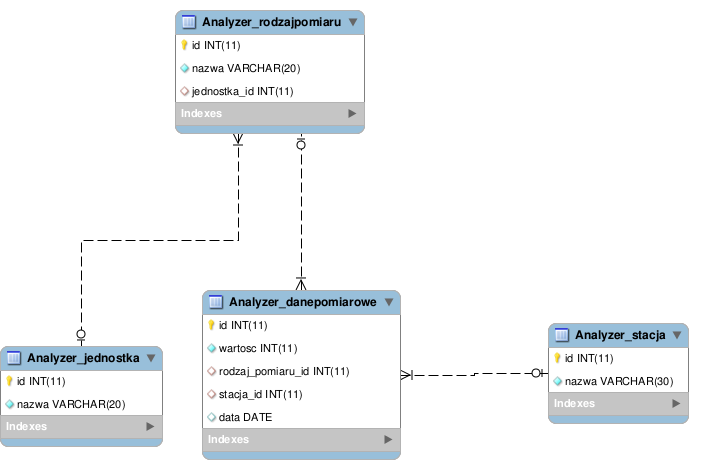
\includegraphics[width=\linewidth]{diagramEER}
\caption{Diagram tabel}
\label{fig:diagramTabel}
\end{figure}

 Poniższa tabela zawiera pełne zestawienie pól stworzonych tabel.
\begin{longtable}{|p{0.25\linewidth}|p{0.25\linewidth}||p{0.5\linewidth}|}
\hline
\textbf{Nazwa tabeli} & \textbf{Nazwa pola} & \textbf{Opis pola} \tabularnewline \hline \hline
\multirow{5}{*}{Analyzer\_danepomiarowe} & id & klucz główny (automatycznie inkrementowany) \tabularnewline\cline{2-3}
 & wartosc & całkowita część danej pomiarowej \tabularnewline\cline{2-3}
 & rodzaj\_pomiaru\_id & klucz obcy (tabela Analyzer\_rodzajpomiaru) \tabularnewline\cline{2-3}
 & stacja\_id & klucz obcy (tabela Analyzer\_stacja)\tabularnewline\cline{2-3}
 & data & data (godzina jest ignorowana) \tabularnewline\hline
\multirow{2}{*}{Analyzer\_jednostka} 
 & id & klucz główny (automatycznie inkrementowany) \tabularnewline\cline{2-3}
 & nazwa & jednostka pomiaru (np. C lub F dla temperatury) \tabularnewline\hline
\multirow{3}{*}{Analyzer\_rodzajpomiaru}
 & id & klucz główny (automatycznie inkrementowany) \tabularnewline\cline{2-3}
 & nazwa & nazwa rodzaju pomiaru, która będzie wykorzystywana do wyboru danych pomiarowych w aplikacji internetowej \tabularnewline\cline{2-3}
 & jednostka\_id & klucz obcy (tabela Analyzer\_jednostka \tabularnewline\hline
\multirow{2}{*}{Analyzer\_stacja}
 & id & klucz główny (automatycznie inkrementowany) \tabularnewline\cline{2-3}
 & nazwa & nazwa stacji, która będzie wykorzystywana do wyboru danych pomiarowych w aplikacji internetowej \tabularnewline\hline
\end{longtable}

\subsection{Opis tabel}
Tabele zostały specjalnie podzielone w taki sposób, aby móc w przyszłości łatwo dodawać kolejne wpisy. Poniżej krótko opisujemy stworzone tabele:
\begin{itemize}
	\item \textbf{Analyzer\_danepomiarowe} - w tabeli tej znajduje się pełne zestawienie danych pomiarowych. Dzięki wykorzystaniu kluczów obcych \textit{ rodzaj\_pomiaru\_id} oraz \textit{stacja\_id} można potem z tabeli filtrować potrzebne dane. Ponieważ w projekcie skupiliśmy się na pomiarach temperatury pole \textit{wartosc} reprezentowane jest przez liczbę całkowitą INT ze znakiem. Kolumna \textit{data} musi zawierać datę wykonania pomiaru, może również być w niej zapisana godzina, aczkolwiek zostanie ona w naszym programie zignorowana. W tej sytuacji można zauważyć, że domyślnie w naszej tabeli znajdują się daty w stylu \verb 2013-12-01  \verb 00:00:00  - godzina wynosi 0. Założyliśmy, że nie będą potrzebne nam pomiary z rozdzielczością godzinową.
	\item \textbf{Analyzer\_jednostka} - jednostka pomiaru została specjalnie wydzielona do osobnej tabeli, ponieważ w bazie może zdarzyć się sytuacja gdy przykładowo stworzony zostanie rodzaj pomiaru TMIN (temperatura minimalna) oraz TMAX (temperatura maksymalna), które mimo, że są różnymi rodzajami pomiaru, posiadają taką samą jednostkę - stopnie Celsjusza. Jednostka może zostać zapisana w maksymalnie 20 znakach, co oczywiście w takim wypadku jest bardzo dużym zapasem. Ponieważ jednostek w przypadku pogody nie będzie dużo nie należy przejmować się, że taka długość napisu może zająć zbyt dużo pamięci w bazie. 
	\item \textbf{Analyzer\_rodzajpomiaru} - rodzajami pomiaru mogą być np. temperatura, ciśnienie, szybkość wiatru itd. Nazwa, która zostanie wpisana w kolumnie \textit{nazwa} będzie widoczna później w aplikacji web. Z tego powodu można wpisać w jej ramach do 20 znaków. Rodzaj pomiaru powiązany jest kluczem obcym z jednostką. Później jest wykorzystywany przy wczytywaniu danych z pliku CSV.
	\item \textbf{Analyzer\_stacja} - tabela przechowuje poza kluczem głównym jedynie nazwy poszczególnych stacji. Na nazwę przyjęliśmy typ VARCHAR(30), czyli może składać się maksymalnie z 30 znaków. Nazwa stacji jest widoczna w aplikacji webowej oraz jest istotna przy wczytywaniu danych z pliku CSV.
\end{itemize}



\section{Użytkownicy}
Ponieważ dane pogodowe pochodzą jedynie od stacji pogodowych, a więc tylko one powinny mieć uprawnienia do wprowadzania pomiarów. Z tego powodu użytkownicy korzystający z bazy danych zostali podzieleni na dwie grupy:
\begin{itemize}
	\item \textbf{użytkownicy anonimowi} - to tacy użytkownicy, którzy mają dostęp jedynie do przeglądania danych pogodowych.
	\item \textbf{użytkownicy zarejestrowani} - to tacy użytkownicy, którzy mają również możliwość dodawania danych pogodowych oraz ich usuwania. Ponieważ każda stacja musi zostać zweryfikowana (aby nie publikowała fałszywych danych) przez administratorów bazy danych, w aplikacji internetowej nie zostało dodane pole rejestracji użytkowników. Zarejestrowani mogą być bezpośrednio przez administratorów poprzez ręczny wpis ich danych potrzebnych do logowania.  
\end{itemize}
Poniżej zamieszczona została tabela zestawiająca funkcję i możliwość korzystania z niej przez poszczególnych użytkowników. Pola oznaczone znakiem X oznaczają, że dany typ użytkownika posiada uprawnienia do wykonywania czynności; w przeciwnym wypadku użytkownik nie ma takiej możliwości.

\begin{longtable}{|p{0.5\linewidth}|p{0.25\linewidth}||p{0.25\linewidth}|}
\hline
\textbf{Funkcja} & \textbf{Anonimowy} & \textbf{Zarejestrowany} \tabularnewline \hline \hline
Wczytanie danych z pliku CSV & - & X \tabularnewline\hline
Usunięcie danych pogodowych & - & X \tabularnewline\hline
Wybór stacji i rodzaju danych pomiarowych & X & X \tabularnewline\hline
Podgląd wykresów pogodowych & X & X \tabularnewline\hline
Podgląd prognozy pogody & X & X \tabularnewline\hline
\end{longtable}


\section{Sprawozdanie z implementacji i dokumentacji}
Projekt był realizowany w zespole 3 osobowym. Aby zapewnić dobry poziom komunikacji między członkami zespołu organizowane były 3 spotkania, w trakcie których omówione zostały kolejno:
\begin{itemize}
	\item Założenia odnośnie tego czym ma być i jakie funkcje ma realizować aplikaca bazo-danowa.
	\item Założenia odnośnie organizacji bazy danych (powiązania między tabelami oraz wybór pakietu django).
	\item Podsumowanie osiągniętych wyników.
\end{itemize}
Poza tym zespół kontaktował się ze sobą na portalu facebook.com na bierząco informując pozostałych członków nt. postępów. Kod został uwspólniony przy użyciu serwisu github.com. 
\newline
Najpierw powstała testowa baza danych, która była wymagana do uruchomienia projektu. Logika została zrealizowana na bazie przykładów dostępnych w internecie. Następnie część logiczna (python i django) została połączona z bazą danych MySQL (odpowiednie modyfikacje pliku settings.py). Aby móc zobaczyć wyniki - działającą stronę należało utworzyć dodatkowo plik analyzer\_main.html oraz w plikach urls.py i views.py powiązać go. W ten sposób udało się uruchomić pierwszy projekt z Django.
\newline
Dostarczając raport nr 1 skorzystaliśmy z gotowej aplikacji, która na podstawie istniejącej już bazy danych generuje diagram tabel. 
Następnie, aby zintegrować bazę danych z logiką i móc korzystać z zawartości bazy wyedytowaliśmy plik models.py, w którym stworzone zostały odpowiednie klasy (modele - odpowiednik tabeli) i dodane do nich odpowiednie pola (poszczególne kolumny tabeli). Obiekt takiej klasy odpowiada jednemu wierszowi tabeli. 
\newline
Prace programistyczne były przeplecione analizą algorytmu ARMA. Po znalezieniu odpowiednich przykładów, wykorzystujących pakiet statsmodels, rozpoczęliśmy w wydzielonym od projektu katalogu testy i próbę stworzenia prognozy pogody. Po kilku testach okazało się, że model ARMA nie był wystarczający do otrzymania sensownej prognozy, a więc postanowiliśmy zaimplementować własny algorytm oparty na modelu ARMA, interpolacji i pewnym wyliczaniu wzmocnień.
\newline
Po skończeniu prac nad prognozą została ona włączona do aplikacji oraz dołączono możliwość logowania użytkownika.
\newline
Na tym etapie zostały przedstawione wyniki w trakcie II spotkania kontrolnego. 
W maju natomiast zostały wprowadzone poprawki w bazie danych oraz stworzony raport końcowy.

\section{Interfejs}
Interfejs graficzny jest tworzony przez Django. Django na podstawie szablonów w postaci plików html oraz danych otrzymanych z funkcji napisanych w python'ie przygotowuje kompletny podgląd strony. 
Strona główna (Rysunek \ref{fig:stronaStartowa}) składa się z 3 dużych przycisków animowanych przy użyciu javascript, które doprowadzają do kolejnych zakładek. W górnej części strony znajdują się przyciski (''Indeks'', ''Podgląd stacji pogodowych'', ''Prognoza'', \textit{''Wczytaj dane''}, ''Autorzy''). W przypadku przycisku ''Wczytaj dane'' nie pojawi się on jeśli użytkownik jest niezalogowany. \newline 
\begin{figure}[p]
	\centering
	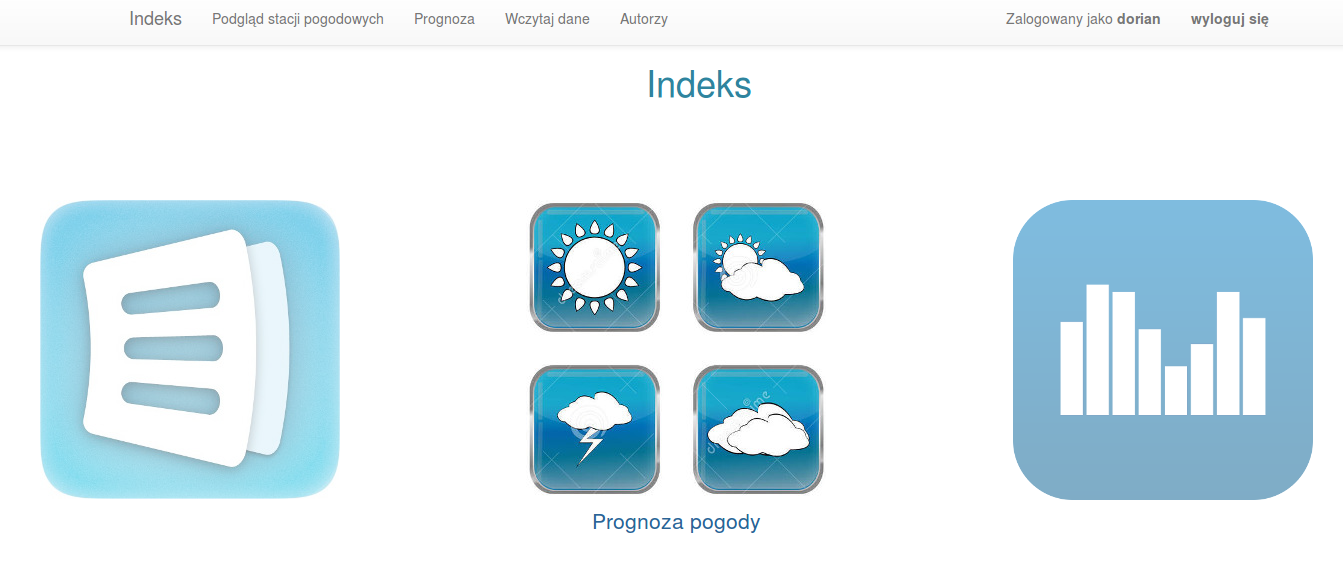
\includegraphics[width=\textheight, angle=90]{000}
	\caption{Strona startowa}
	\label{fig:stronaStartowa}
	\end{figure}

Po kliknięciu na zakładki ''Podgląd stacji pogodowych'' oraz ''Prognoza'' otwiera się bardzo podobna podstrona (Rysunek \ref{fig:podgladStacji}), która służy do wyboru rodzaju pomiaru oraz stacji, dla której dane mają zostać wyrysowane. W przypadku zalogowanych użytkowników pojawia się również możliwość skasowania danych w postaci przycisku ''delete''. 
\newline
\begin{figure}[p]
	\centering
	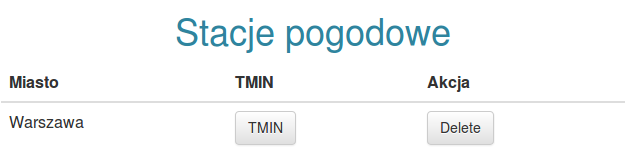
\includegraphics[width=\linewidth]{001}
	\caption{Podgląd stacji pogodowych - użytkownik zalogowany}
	\label{fig:podgladStacji}
	\end{figure}

Wykresy rysowane są przy użyciu biblioteki matplotlib (Rysunek \ref{fig:wykres}). 
\newline
\begin{figure}[p]
	\centering
	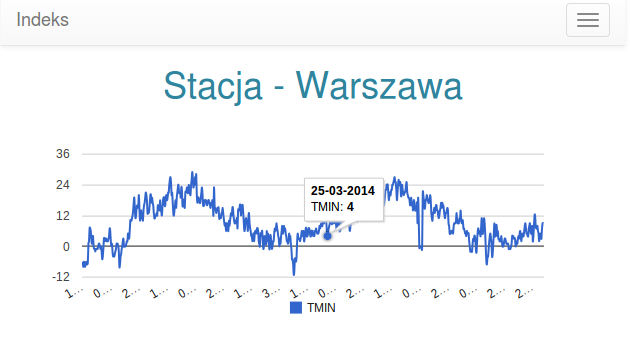
\includegraphics[width=\linewidth]{002}
	\caption{Wyrysowany wykres}
	\label{fig:wykres}
	\end{figure}



\section{Instrukcja obsługi}
\subsection{Instalacja bazy danych}
Baza danych została wdrożona na systemie Linux (przetestowana na dystrybucjach Ubuntu oraz Mint). Aby móc ją uruchomić należy wcześniej zainstalować poniższe pakiety:
\begin{itemize}
	\item python2.7
	\item python-numpy
	\item python-scipy
	\item python-matplotlib
	\item ipython
	\item ipython-notebook
	\item python-pandas
	\item python-sympy
	\item python-nose
	\item python-statsmodels
	\item python-tk
	\item mysql-connector-python
	\item django-pandas
	\item django-model-utils
	\item scipy
	\item mysql-server
\end{itemize}
Następnie koniecznie należy zaimportować bazę danych poprzez wywołanie poniższej komendy w terminalu w folderze głównym aplikacji (zawierający plik requirements.txt oraz manage.py):
\begin{verbatim}
	python2 manage.py migrate
\end{verbatim}

\subsection{Przygotowanie plików wejściowych}
Ponieważ aplikacja webowa nie pobiera sama danych pogodowych z internetu, należy je załadować z pliku. Aby móc to zrobić trzeba przygotować plik CSV zawierający komplet wymaganych informacji.
W kolejnych wierszach pliku muszą się znaleźć kolejne pomiary. W kolejnych wierszach należy pola oddzielić przecinkami:
	\begin{verbatim}
		nazwa_stacji,data_RRRRMMDD,rodzaj_pomiaru,wartosc_pomiaru
	\end{verbatim}
W przypadku pola \verb data_RRRRMMDD  data musi zostać zapisana w postaci ciągu cyfr nieoddzielonych żadnymi separatorami. Przykładowa zawartość pliku:
	\begin{verbatim}
		Warszawa,20130118,TMIN,-6
		Warszawa,20130119,TMIN,-8
		Warszawa,20130120,TMIN,-6
		Warszawa,20130121,TMIN,-7
	\end{verbatim}

Następnie należy ręcznie zarejestrować rodzaj pomiaru. Zostało to pozostawione stronie administracyjnej, ponieważ wiąże się to bezpośrednio z początkowym wdrażaniem bazy na serwerze. 
W tym celu należy dodać wpisy w odpowiednich tabelach:
\begin{itemize}
	\item \textbf{Analyzer\_jednostka} - dodać opis słowny i ID jednostki związanej z mierzoną cechą
	\item \textbf{Analyzer\_rodzajpomiaru} - dodać opis słowny zgodny z polem \verb rodzaj_pomiaru  z pliku CSV, nadać numer ID oraz odwołać się do klucza wpisanej przed chwilą jednostki
	\item \textbf{Analyzer\_stacja} - dodać nazwę stacji zgodnie z polem \verb nazwa_stacji  z pliku CSV oraz nadać jej numer ID.
\end{itemize}

\subsection{Pierwsze uruchomienie bazy}
Skonfigurowana baza danych wymaga jedynie uruchomienia środowiska, w którym będzie działać aplikacja internetowa. 
W tym celu (przy założeniu, że wszystkie zależności zostały wcześniej zainstalowane) należy stworzyć środowisko:
\begin{verbatim}
	virtualenv --no-site-packages env
	source env/bin/activate
	pip2 install -r requirements.txt --allow-external mysql-connector-python pandas scipy statsmodels django-pandas django-model-utils
\end{verbatim}
Aby uruchomić teraz bazę danych wystarczy:
\begin{verbatim}
	python2 manage.py runserver
\end{verbatim}
I następnie podany w konsoli adres strony skopiować i wkleić w przeglądarce internetowej (domyślnie: \verb http://127.0.0.1:8000/ ).

\subsection{Kolejne uruchomienie bazy}
Przy każdym kolejnym uruchomieniu bazy wystarczy ponownie uruchomić środowisko i serwer:
\begin{verbatim}
	source env/bin/activate
	python2 manage.py runserver
\end{verbatim}
oraz znowu skopiować adres i wkleić go do przeglądarki internetowej. 





\end{document}
